% !TeX program = xelatex
% UTF-8. Compile twice with XeLaTeX, or once with Tectonic (automatic reruns).
\documentclass[UTF8,12pt,a4paper,fontset=fandol]{ctexart}
\usepackage[a4paper,top=2.5cm,bottom=2.5cm,left=2.6cm,right=2.4cm]{geometry}
\usepackage{amsmath,amssymb,graphicx,booktabs,longtable,array}
\graphicspath{{figures/}{../results/}}
\usepackage{caption,placeins,fancyhdr,xurl,float}
\usepackage[unicode,hidelinks]{hyperref}
\hypersetup{hypertexnames=false,pdftitle={基于不同文本表示的 NYT 新闻分类实验},pdfauthor={程子涵},pdfsubject={作业一 文本分类实验报告}}
\urlstyle{same}
\setlength{\parindent}{2em}
\setlength{\parskip}{0.3em}
\linespread{1.30}
\setlength{\emergencystretch}{3em}
\clubpenalty=10000
\widowpenalty=10000
\setlength{\headheight}{15pt}
\pagestyle{fancy}
\fancyhf{}
\fancyhead[C]{\small NYT 新闻分类实验报告}
\fancyfoot[C]{\thepage}
\renewcommand{\headrulewidth}{0pt}
\renewcommand{\footrulewidth}{0pt}
\fancypagestyle{plain}{\fancyhf{}\fancyfoot[C]{\thepage}\renewcommand{\headrulewidth}{0pt}}
\ctexset{section={format=\Large\bfseries,beforeskip=1.2em,afterskip=0.8em},subsection={format=\large\bfseries,beforeskip=1em,afterskip=0.5em},paragraph={format=\normalsize\bfseries,runin=false,beforeskip=0.5em,afterskip=0.2em}}
\captionsetup{font=small,labelfont=bf,justification=centering}
\setcounter{tocdepth}{2}
\newlength{\TableWidth}
\begin{document}
\begin{titlepage}
\centering
\vspace*{1.3cm}
{\Large 课程作业实验报告\par}
\vspace{2cm}
{\huge\bfseries 基于不同文本表示的\\[0.6em]NYT 新闻分类实验\par}
\vspace{0.8cm}
{\large 词袋模型\quad 平均词向量\quad BERT 微调\par}
\vspace{0.5cm}
{\large 作业一\par}
\vspace{2.4cm}
{\large
姓名：程子涵\par\vspace{0.7em}
学号：2413921\par\vspace{0.7em}
班级：物联网工程班\par}
\vspace{1cm}
任务类型：英文新闻三分类\par
评价指标：Accuracy 与 Macro-F1\par
\vfill
\end{titlepage}
\clearpage
\pagenumbering{Roman}
\section*{摘要}
\phantomsection
\addcontentsline{toc}{section}{摘要}
本文在 NYT 新闻三分类任务上比较 Binary BoW、Word Frequency、GloVe、基于 AG News 和 NYT 的 Word2Vec，以及 BERT 微调六种方法。五种传统表示均结合 Logistic Regression，六组实验共用去重后的 80\% / 10\% / 10\% 数据划分，以 Accuracy 和 Macro-F1 评价分类效果，并结合词向量覆盖率、分类别 F1、混淆矩阵和训练曲线进行分析。

在固定随机种子和预设参数下，GloVe 的测试 Accuracy 为 0.9852，Macro-F1 为 0.9601，均为六组最高；Word Frequency 和 BERT 的 Macro-F1 分别为 0.9572 和 0.9525。目标领域 NYT Word2Vec 优于外部 AG News Word2Vec。错误主要集中在 business 与 politics 之间，说明类别边界交叉仍是主要困难。结果表明，文本表示、领域匹配和实验约束共同影响分类表现；本研究仅基于单次固定划分，尚不能给出统计显著性或普遍最优结论。

关键词：新闻分类；词袋模型；GloVe；Word2Vec；BERT；Macro-F1

\clearpage
\tableofcontents
\clearpage
\pagenumbering{arabic}
\FloatBarrier
\section{引言}
新闻分类将非结构化文本映射为离散主题标签，是检验文本表示有效性的一种直接方式。稀疏词袋强调词汇分布，平均词向量引入连续语义表示，BERT 则通过上下文编码学习任务相关特征。本实验在统一数据划分与评价协议下，观察这些表示方式在同一目标任务上的表现差异。

本实验按照作业要求，在 NYT 新闻三分类任务上比较两种词袋表示、三种 100 维词向量表示和 BERT 微调，共六组方法。传统方法使用 Logistic Regression，所有方法使用相同的数据划分，以测试集 Accuracy 和 Macro-F1 评价。

在本次固定划分和参数设置下，GloVe 的测试 Accuracy 为 0.9852、Macro-F1 为 0.9601，均为六组最高；Word Frequency 的 Macro-F1 为 0.9572，BERT 为 0.9525。复杂模型在本实验条件下没有必然优势。该结论仅描述本次运行，不代表多次随机实验的统计显著性结论。

\FloatBarrier
\section{数据与实验协议}
原始 NYT 含 11,519 条记录。预处理先删除 72 条完全相同的重复文本，保留首次出现的记录，得到 11,447 条；若重复文本标签冲突则停止运行。原始 CSV 未被改写。去重是防止同一文本跨集合出现的额外处理，作业文档未明确要求；因此报告明确披露样本数量变化。

使用 NumPy RandomState(42) 随机打乱去重后的样本，再按 80\% / 10\% / 10\% 划分。训练集和验证集数量向下取整，余数归测试集。采用普通随机划分而非分层抽样；六组实验共享原始行号清单，三对集合间完全相同文本交集均为 0。

\begin{table}[H]
\centering
\caption{数据划分与类别分布}\label{tab:1}
\small
\setlength{\tabcolsep}{5pt}
\setlength{\TableWidth}{\dimexpr\linewidth-10\tabcolsep\relax}
\renewcommand{\arraystretch}{1.3}
\begin{tabular}{>{\raggedright\arraybackslash}p{0.20\TableWidth}>{\raggedright\arraybackslash}p{0.19\TableWidth}>{\raggedright\arraybackslash}p{0.19\TableWidth}>{\raggedright\arraybackslash}p{0.19\TableWidth}>{\raggedright\arraybackslash}p{0.23\TableWidth}}
\toprule
\textbf{集合} & \textbf{business} & \textbf{politics} & \textbf{sports} & \textbf{合计} \\
\midrule
训练集 & 1148 & 1143 & 6866 & 9157 \\
验证集 & 140 & 148 & 856 & 1144 \\
测试集 & 129 & 142 & 875 & 1146 \\
\bottomrule
\end{tabular}
\end{table}
AG News 共 90,000 条文本，仅用于外部 Word2Vec 的无监督训练。NYT Word2Vec 仅使用 NYT 训练集学习词向量，词袋词表亦仅由训练集建立，验证集与测试集不参与特征学习或分类器拟合。

所有超参数预先固定，验证集用于监测和报告；未进行验证集网格搜索，也未合并 train+val 重训。作业未要求这两项操作。测试集仅用于最终评价，不根据测试得分回调参数。

\subsection{评价指标}
Accuracy 为正确分类数占测试样本数的比例。每类 F1 由精确率 $P$ 与召回率 $R$ 计算，Macro-F1 为三个类别 F1 的算术平均。
\begin{equation}
\mathrm{Accuracy}=\frac{N_{\mathrm{correct}}}{N_{\mathrm{test}}},\qquad F_{1,c}=\frac{2P_cR_c}{P_c+R_c},\qquad \mathrm{Macro}\text{-}F_1=\frac{1}{3}\sum_{c=1}^{3}F_{1,c}.
\end{equation}
测试集 sports 占 76.35\%，因此同时报告 Macro-F1 和分类别指标以避免多数类掩盖少数类误差。

\FloatBarrier
\section{方法与参数设置}
传统方法采用“分词—文档表示—逻辑回归—类别预测”的统一流程，BERT 使用“预训练分词—上下文编码—分类头微调”的流程。统一划分保证各方法面对相同样本；表示维度、预训练语料和输入长度仍存在差异，因此比较反映的是本次完整配置下的实际表现。

\subsection{词袋表示与逻辑回归}
Binary BoW 用 \path{0/1} 表示词是否出现；Word Frequency 使用原始出现次数，不做 TF-IDF 加权或长度归一化。两者训练词表大小均为 65,902，采用稀疏矩阵保存文档向量。作业明确列出两种方法，本实验完成这两项。

Task 1 和 Task 2 统一先小写化，再用正则 [a-zA-Z]+(?:'[a-zA-Z]+)?|\textbackslash{}d+ 分词，保留英文词、词内撇号和数字。不依赖 NLTK 或 punkt，避免跨环境自动切换分词器；作业对 NLTK 的表述为可考虑使用。BERT 使用其预训练 tokenizer。

五组传统模型均采用 LogisticRegression：C=1.0、solver=lbfgs、L2 正则、\path{max_iter}=2000、\path{random_state}=42、\path{class_weight}=None。未额外重采样或类别加权。五组实际迭代数依次为 20、122、57、34、27，日志均确认收敛；迭代上限本身不保证收敛。

\subsection{平均词向量表示}
设文档中能够查到向量的词出现序列为 $V(d)$，词向量为 $\mathbf{e}(w)$，则文档表示为
\begin{equation}
\mathbf{v}(d)=\frac{1}{|V(d)|}\sum_{w\in V(d)}\mathbf{e}(w).
\end{equation}
这种表示将文档压缩为固定的 100 维向量，便于复用同一分类器；同时，平均操作不保留词序，也会削弱少量关键词与长距离关系的影响。该性质用于解释表示能力的差异，不等于对具体错误样本的模型归因。

预训练 GloVe 使用 glove.6B.100d.txt，共 400,000 个词，每词 100 维。对每篇文档中可查到词向量的所有词出现取算术平均，重复词按出现次数参与平均；未登录词跳过，若无有效词则返回全零向量。本次三组词向量实验在三个集合中均无全零文档。

\begin{table}[H]
\centering
\caption{Word2Vec 训练配置}\label{tab:2}
\small
\setlength{\tabcolsep}{5pt}
\setlength{\TableWidth}{\dimexpr\linewidth-6\tabcolsep\relax}
\renewcommand{\arraystretch}{1.3}
\begin{tabular}{>{\raggedright\arraybackslash}p{0.28\TableWidth}>{\raggedright\arraybackslash}p{0.36\TableWidth}>{\raggedright\arraybackslash}p{0.36\TableWidth}}
\toprule
\textbf{项目} & \textbf{Word2Vec AG} & \textbf{Word2Vec NYT} \\
\midrule
训练语料 & AG News 全部文本 & NYT 训练集 \\
文档数 & 90,000 & 9,157 \\
向量维度 & 100 & 100 \\
词表大小 & 23,529 & 29,066 \\
模型与窗口 & Skip-gram / window=5 & Skip-gram / window=5 \\
最低词频与轮数 & \path{min_count}=5 / epochs=10 & \path{min_count}=5 / epochs=10 \\
\bottomrule
\end{tabular}
\end{table}
两组 Word2Vec 其余参数一致：negative=5、hs=0、sample=0.001、alpha=0.025、\path{min_alpha}=0.0001、seed=42、workers=1、\path{ns_exponent}=0.75、\path{sorted_vocab}=1、\path{shrink_windows}=True、\path{batch_words}=10000；使用稳定 SHA256 词哈希减小跨进程随机性。

\subsection{BERT 微调}
模型为 google-\path{bert/bert-base-uncased}；\path{max_length}=64，包含特殊 token，超长文本截断，不足长度补齐。训练 3 epochs，训练和评价 \path{batch_size}=16，AdamW，初始学习率 2e-5，\path{weight_decay}=0.01，线性学习率衰减，无 warmup。随机种子和 \path{data_seed} 均为 42，启用 \path{full_determinism}。

每轮结束评价验证集，完整训练第 3 轮后保存模型和 tokenizer，并使用该最终模型评价测试集。运行设备为 Colab Tesla T4，累计 1,719 个优化步骤，实际完成 3.0 epochs。

\clearpage
\FloatBarrier
\section{实验结果与比较}
\begin{table}[H]
\centering
\caption{六组方法的验证集与测试集结果}\label{tab:3}
\small
\setlength{\tabcolsep}{5pt}
\setlength{\TableWidth}{\dimexpr\linewidth-10\tabcolsep\relax}
\renewcommand{\arraystretch}{1.3}
\begin{tabular}{>{\raggedright\arraybackslash}p{0.28\TableWidth}>{\raggedright\arraybackslash}p{0.18\TableWidth}>{\raggedright\arraybackslash}p{0.18\TableWidth}>{\raggedright\arraybackslash}p{0.18\TableWidth}>{\raggedright\arraybackslash}p{0.18\TableWidth}}
\toprule
\textbf{方法} & \textbf{验证 Acc} & \textbf{验证 F1} & \textbf{测试 Acc} & \textbf{测试 F1} \\
\midrule
Binary BoW & 0.9808 & 0.9529 & 0.9808 & 0.9478 \\
Word Frequency & 0.9816 & 0.9570 & 0.9825 & 0.9572 \\
GloVe & 0.9764 & 0.9423 & 0.9852 & 0.9601 \\
Word2Vec AG & 0.9650 & 0.9166 & 0.9738 & 0.9335 \\
Word2Vec NYT & 0.9747 & 0.9392 & 0.9817 & 0.9566 \\
BERT & 0.9747 & 0.9444 & 0.9791 & 0.9525 \\
\bottomrule
\end{tabular}
\end{table}
\begin{figure}[H]
\centering
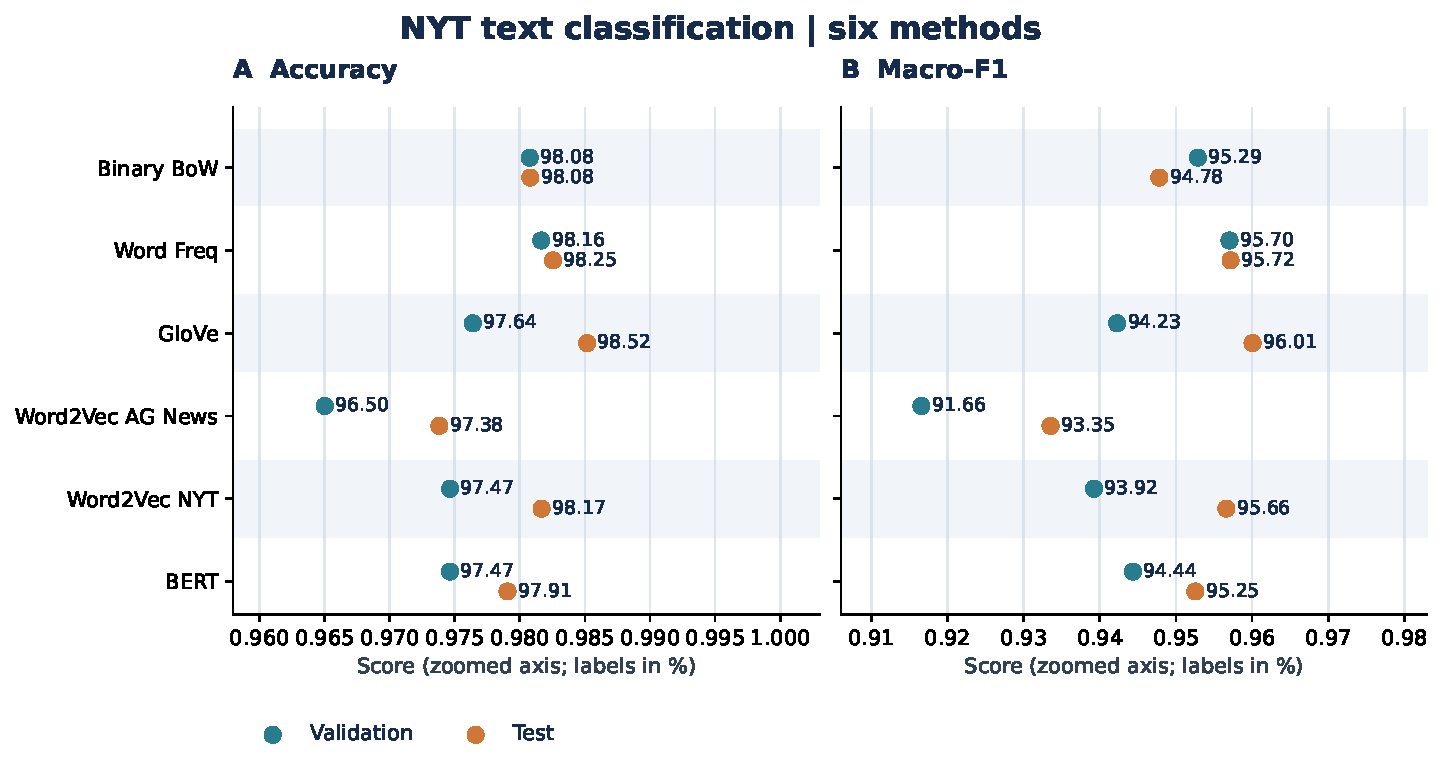
\includegraphics[width=\linewidth]{comparison_chart.pdf}
\caption{六组方法的验证集与测试集指标。F1 为 Macro-F1，点旁数字为百分数，横轴局部放大以便观察差异。}
\label{fig:comparison_chart}
\end{figure}
Word Frequency 相比 Binary BoW，测试 Accuracy 提高 0.17 个百分点，Macro-F1 提高 0.94 个百分点，说明在本次数据上保留词频比只保留是否出现略有优势。两者都保留了完整文档的词汇统计，但不表达词序。

GloVe 比 Word Frequency 的测试 Accuracy 高 0.26 个百分点，Macro-F1 高 0.29 个百分点，差异较小，不能仅据一次运行断言普遍优越。GloVe 的测试得分高于验证得分反映了集合样本组成差异，不能据此认定验证集参与了训练。

本次 BERT 测试 Accuracy 为 0.9791、Macro-F1 为 0.9525，低于 GloVe 和 Word Frequency。长度上限 64 限制了可见上下文，而词袋与词向量方法处理全文；这一差异可能影响表现，但尚无长度消融实验，不能视为已证实的因果解释。

\FloatBarrier
\section{词向量覆盖率与分类别表现}
\begin{table}[H]
\centering
\caption{词向量的 token 覆盖率}\label{tab:4}
\small
\setlength{\tabcolsep}{5pt}
\setlength{\TableWidth}{\dimexpr\linewidth-8\tabcolsep\relax}
\renewcommand{\arraystretch}{1.3}
\begin{tabular}{>{\raggedright\arraybackslash}p{0.28\TableWidth}>{\raggedright\arraybackslash}p{0.24\TableWidth}>{\raggedright\arraybackslash}p{0.24\TableWidth}>{\raggedright\arraybackslash}p{0.24\TableWidth}}
\toprule
\textbf{表示方法} & \textbf{训练词覆盖率} & \textbf{验证词覆盖率} & \textbf{测试词覆盖率} \\
\midrule
GloVe & 98.18\% & 98.14\% & 98.15\% \\
Word2Vec AG & 95.79\% & 95.83\% & 95.92\% \\
Word2Vec NYT & 98.90\% & 98.54\% & 98.55\% \\
\bottomrule
\end{tabular}
\end{table}
覆盖率按 token 出现次数计算，不是独立词种比例。NYT Word2Vec 的测试词覆盖率为 98.55\%，高于 AG Word2Vec 的 95.92\%；前者 Macro-F1 高 2.31 个百分点。尽管 AG 文档数更多，其领域和文本长度不同，文档数并不等于有效词规模，结果与目标领域匹配的重要性一致。

GloVe 的测试覆盖率为 98.15\%，略低于 NYT Word2Vec，但 Macro-F1 更高，说明覆盖率不能单独解释效果。预训练语料规模、向量质量以及平均池化对语义信息的损失都可能影响分类。

\begin{figure}[H]
\centering
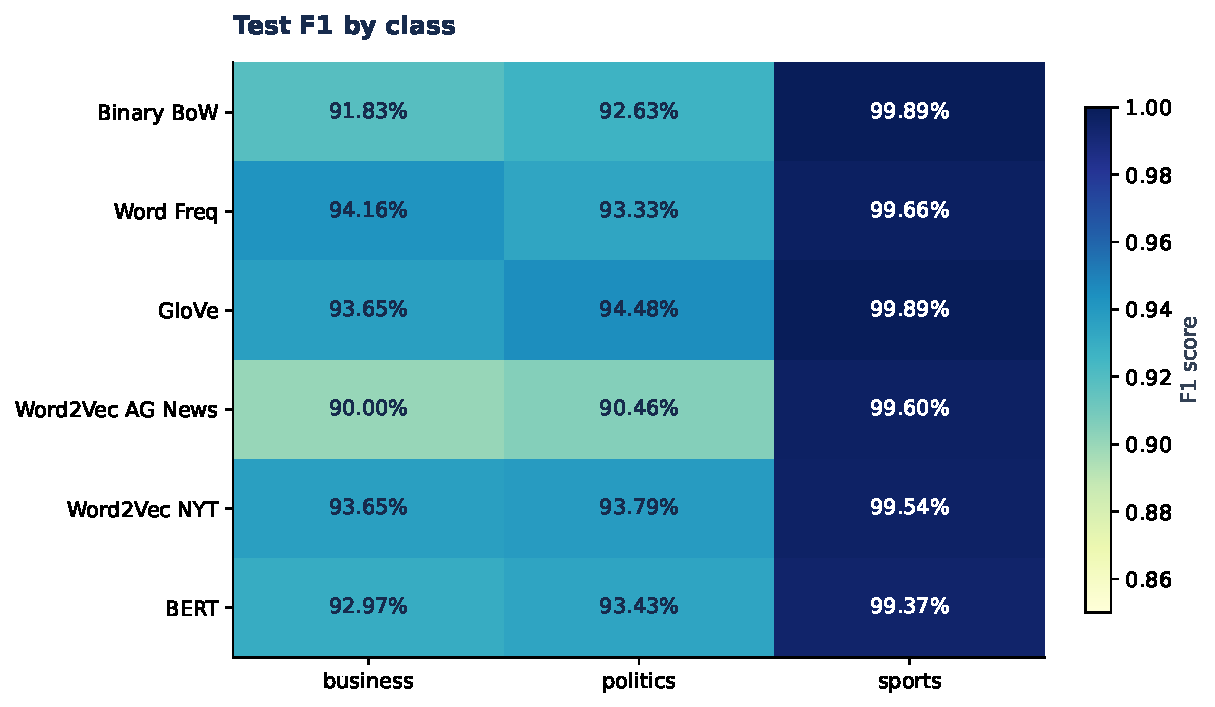
\includegraphics[width=\linewidth]{class_f1_chart.pdf}
\caption{各方法在测试集上的分类别 F1。固定色阶为 0.85 至 1.00，单元格显示百分数。}
\label{fig:class_f1_chart}
\end{figure}
六种方法在 sports 上的 F1 均超过 0.993，而 business 与 politics 的 F1 约为 0.900 至 0.945。sports 样本占比高且主题词明显，整体 Accuracy 因而高于 Macro-F1。Word Frequency 的 business F1 为 0.9416，高于 GloVe 的 0.9365；GloVe 在 politics 和 sports 上更好，最终获得更高的平均 F1。

\FloatBarrier
\section{BERT 训练过程与运行环境}
\begin{figure}[H]
\centering
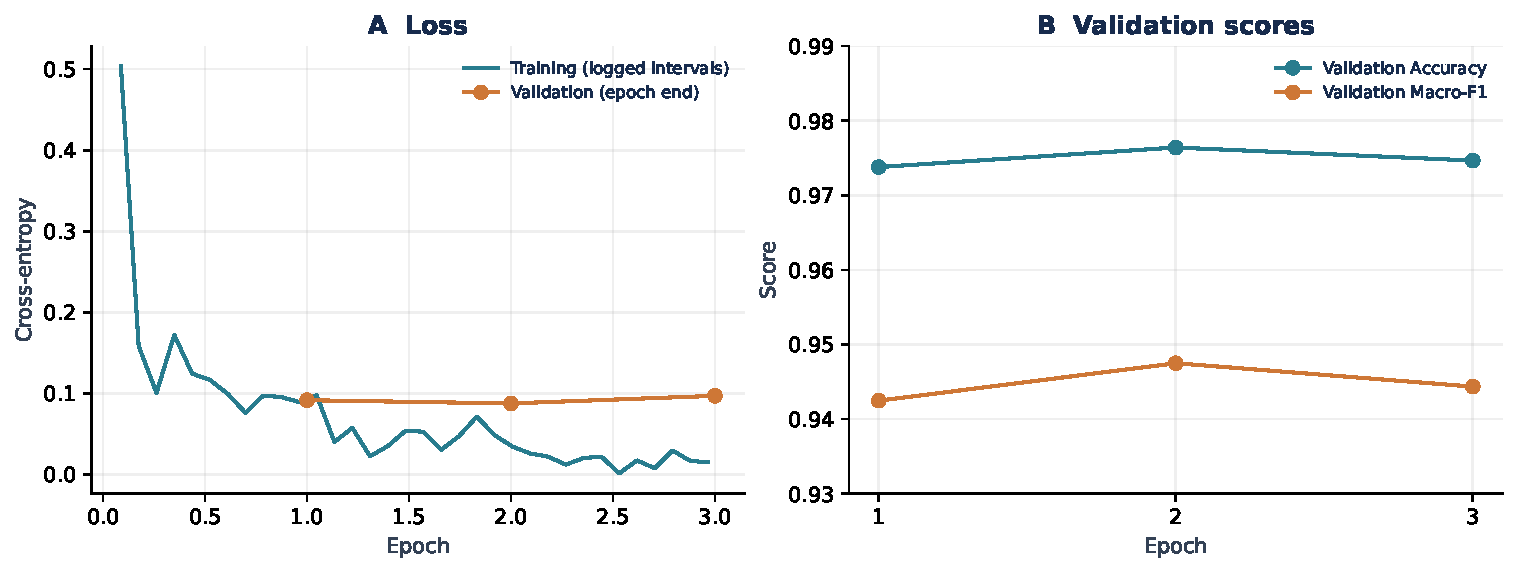
\includegraphics[width=\linewidth]{bert_training_curve.pdf}
\caption{BERT 的训练日志与轮末验证指标。训练 loss 为日志区间平均，验证 loss 为完整验证集评价，两者采样粒度不同。}
\label{fig:bert_training_curve}
\end{figure}
\begin{table}[H]
\centering
\caption{BERT 各轮验证指标}\label{tab:5}
\small
\setlength{\tabcolsep}{5pt}
\setlength{\TableWidth}{\dimexpr\linewidth-8\tabcolsep\relax}
\renewcommand{\arraystretch}{1.3}
\begin{tabular}{>{\raggedright\arraybackslash}p{0.17\TableWidth}>{\raggedright\arraybackslash}p{0.27\TableWidth}>{\raggedright\arraybackslash}p{0.28\TableWidth}>{\raggedright\arraybackslash}p{0.28\TableWidth}}
\toprule
\textbf{Epoch} & \textbf{验证 Loss} & \textbf{验证 Accuracy} & \textbf{验证 Macro-F1} \\
\midrule
1 & 0.0917 & 0.9738 & 0.9425 \\
2 & 0.0877 & 0.9764 & 0.9475 \\
3 & 0.0971 & 0.9747 & 0.9444 \\
\bottomrule
\end{tabular}
\end{table}
训练 loss 整体下降，第 2 轮验证 Macro-F1 为 0.9475，第 3 轮降为 0.9444，同时验证 loss 回升。这提示可能出现轻度过拟合，也可能包含单次训练波动。实验仍按预先约定使用第 3 轮模型，没有依据测试集或验证集改选轮次。

\begin{table}[H]
\centering
\caption{各方法日志总耗时与执行环境}\label{tab:6}
\small
\setlength{\tabcolsep}{5pt}
\setlength{\TableWidth}{\dimexpr\linewidth-6\tabcolsep\relax}
\renewcommand{\arraystretch}{1.3}
\begin{tabular}{>{\raggedright\arraybackslash}p{0.30\TableWidth}>{\raggedright\arraybackslash}p{0.26\TableWidth}>{\raggedright\arraybackslash}p{0.44\TableWidth}}
\toprule
\textbf{方法} & \textbf{日志总耗时 秒} & \textbf{执行环境} \\
\midrule
Binary BoW & 6.99 & Windows / CPU \\
Word Frequency & 16.36 & Windows / CPU \\
GloVe & 30.38 & Windows / CPU \\
Word2Vec AG & 329.31 & Windows / CPU \\
Word2Vec NYT & 456.20 & Windows / CPU \\
BERT & 466.35 & Colab / Tesla T4 \\
\bottomrule
\end{tabular}
\end{table}
总耗时为 Experiment 初始化后至结果保存期间的计时，包含特征构建、训练及输出等开销，不等同于纯训练时间；数据划分发生在计时之前。BERT 的训练段耗时为 414.31 秒。CPU 和 GPU 平台、软件版本及初始化开销不同，表中耗时只能说明本次运行成本，不能直接比较算法速度。

传统方法环境：Python 3.13.9、NumPy 2.3.5、pandas 2.3.3、scikit-learn 1.7.2、gensim 4.4.0。BERT 环境：Python 3.13.15、PyTorch 2.11.0+cu128、CUDA 12.8、transformers 4.56.2、accelerate 1.10.1、scikit-learn 1.6.1。完整依赖版本随每次实验保存。

\clearpage
\FloatBarrier
\section{混淆矩阵与错误分析}
\begin{figure}[H]
\centering
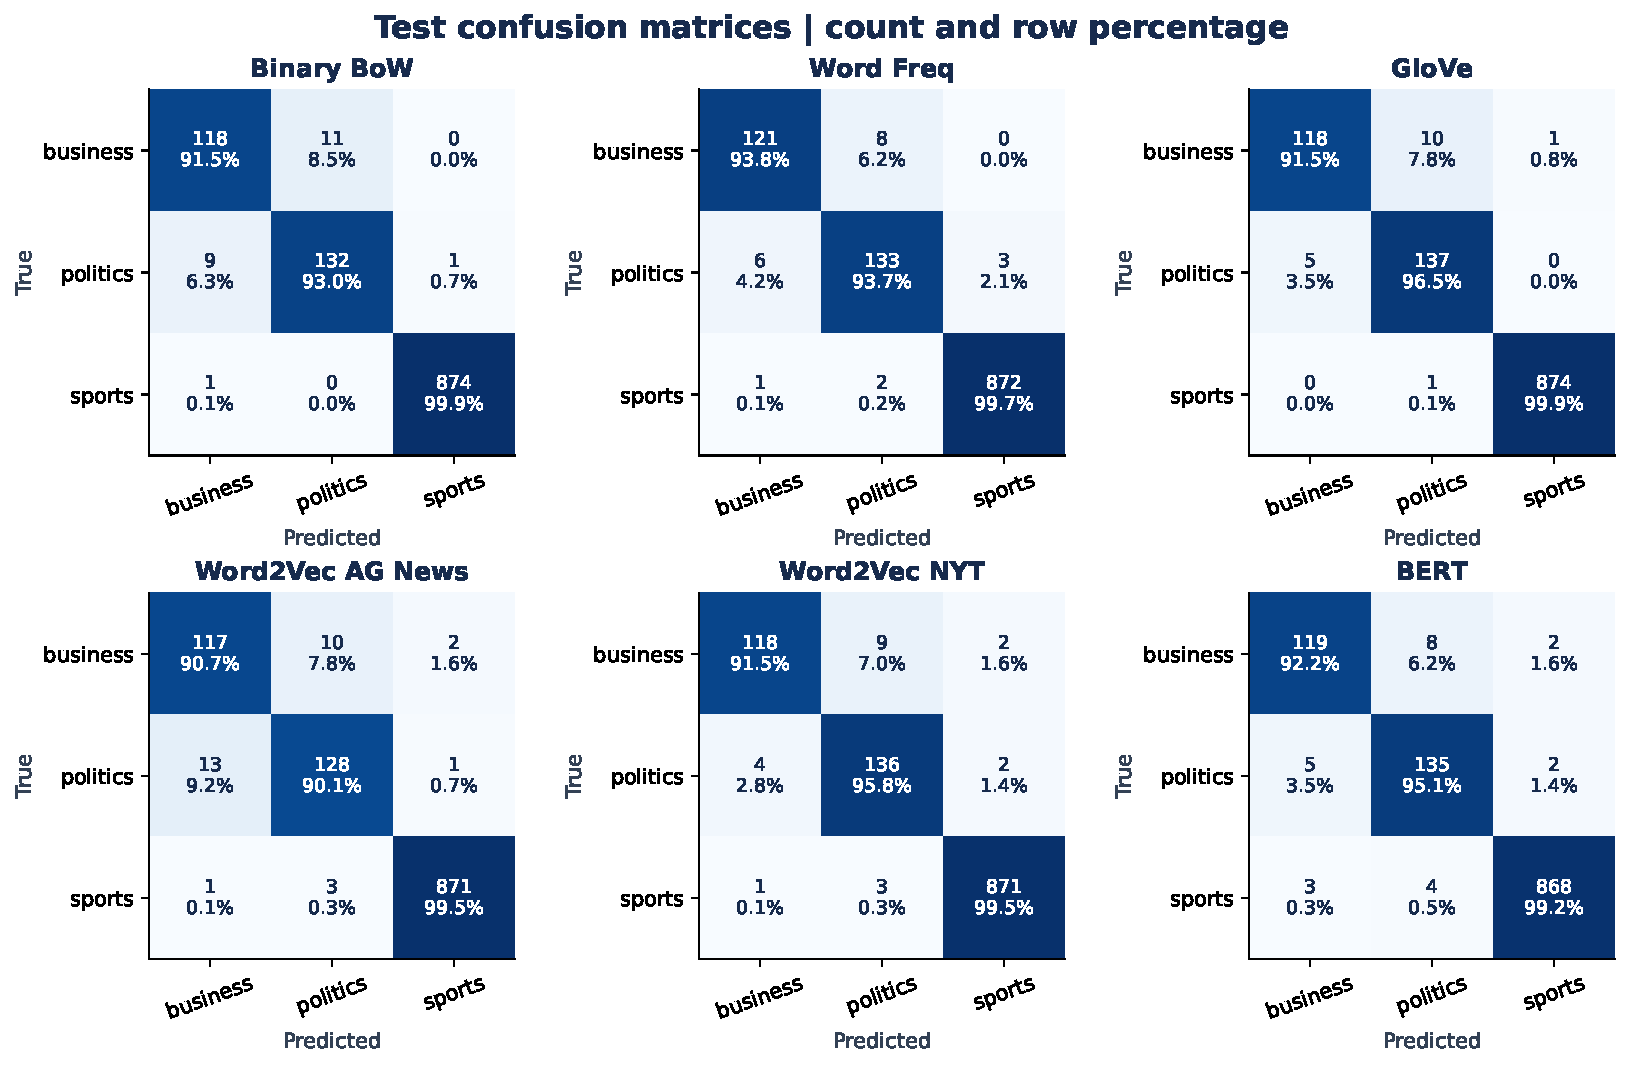
\includegraphics[width=\linewidth]{confusion_matrices.pdf}
\caption{六种方法的测试混淆矩阵。行为真实类别，列为预测类别；数字同时列出样本数及行归一化百分比。}
\label{fig:confusion_matrices}
\end{figure}
六组方法错误数依次为 22、20、17、30、21、24。GloVe 的 17 个错误中，business$\rightarrow$politics 为 10 个、politics$\rightarrow$business 为 5 个，二者合计占 88.24\%；BERT 的对应交叉误判共 13 个，占其 24 个错误的 54.17\%。商业与政策主题交叉是主要困难，但 BERT 还存在更多涉及 sports 的错误。

\subsection{可追溯错误案例}
原始 CSV 数据行 \path{source_row}=8022（从 0 起计，不含表头）：报道联邦预算削减对机场和航班的影响，真实类别为 politics，GloVe 和 BERT 均预测为 business。政府预算与航空业经营词汇同时出现，主题边界具有交叉性。

\path{source_row}=11007：报道警方拘捕从事投资风险调查的咨询人士，真实类别为 business，GloVe 预测为 politics。警方、逮捕等词语可能强化政治或公共事务信号，而商业调查背景决定了原始标签。

\path{source_row}=8246：报道以万亿美元硬币应对债务上限的讨论，真实类别为 business，BERT 预测为 politics。白宫与国会冲突和经济政策在同一文本中交织。以上为结合文本的定性解释，不等于已经验证的模型归因。完整原文及预测见各实验 \path{test_errors.csv}。

\FloatBarrier
\section{总结与讨论}
\subsection{主要结论与研究限制}
本次结果表明，传统词汇特征已能很好地区分 NYT 三类新闻；100 维平均 GloVe 在固定实验条件下取得最高测试指标。使用 NYT 训练语料学习 Word2Vec，比使用 AG News 得到更好的目标任务效果；BERT 在 64 token、3 epochs 的约束下没有超过最佳传统方法。

实验的限制包括：只使用一次固定随机划分和一个随机种子，没有置信区间或显著性检验；没有超参数搜索、类别加权对照和 BERT 长度消融；完全重复文本去重不能排除语义相近新闻。

\subsection{实验思考}
\paragraph*{1.模型复杂不一定效果更好。}\mbox{}\par\nopagebreak
这次实验中，GloVe 的测试集指标最高，BERT 没有超过它。我觉得模型效果不只取决于模型有多复杂，也和任务特点、文本长度以及数据规模有关。对于新闻分类，许多类别本身就有比较明显的词汇特征，传统方法也能取得不错的结果。

\paragraph*{2.不能只看 Accuracy。}\mbox{}\par\nopagebreak
测试集中 sports 样本比 business 和 politics 多得多，因此模型即使主要分对了 sports，也可能得到较高的 Accuracy。结合 Macro-F1 和各类别 F1 后，可以看到 business 和 politics 更容易被混淆，模型在少数类别上的表现需要单独关注。

\paragraph*{3.文本表示方式会影响模型能捕捉到的信息。}\mbox{}\par\nopagebreak
Binary BoW 只记录词是否出现，Word Frequency 还保留词语出现次数，平均词向量则把词语映射到连续空间。这些表示各有侧重。实验中 Word Frequency 略好于 Binary BoW，也让我看到词频信息确实可能对分类有帮助，不过不同方法之间的差距还需要结合具体数据来理解。

\paragraph*{4.有些分类错误来自新闻主题交叉。}\mbox{}\par\nopagebreak
错误案例中，有的文章同时讨论政府政策和商业影响，模型把真实的 business 文章预测为 politics，或反过来。这些新闻的主题边界并不总是清楚，分类错误不一定只是模型没有学好，也可能说明标签体系和文本内容存在交叉。

\paragraph*{5.实验结论依赖公平、可追溯的比较。}\mbox{}\par\nopagebreak
所有方法使用相同的数据划分，训练参数和预测结果也有记录，这让我能更有依据地比较模型。如果每种方法采用不同的数据划分，结果差异就可能来自数据本身，而不是模型。

\paragraph*{6.一次结果还不足以说明普遍规律。}\mbox{}\par\nopagebreak
这次实验使用固定随机种子和一份数据划分，得出的结论只适用于当前实验设置。若继续研究，我想尝试不同随机种子，并调整 BERT 的最大文本长度，观察结果是否稳定，以及较长文本是否能改善分类表现。

\subsection{后续研究方向}
后续可在保持数据划分协议和测试集独立性的前提下，使用多个随机种子重复实验，报告均值与波动范围；对 BERT 输入长度进行受控对比，以检验截断是否影响效果；针对 business 与 politics 的交叉样本进一步检查文本与标签边界。这些均属于待开展的扩展研究，不计入本次实验结果。

\FloatBarrier
\section*{参考资料}
\phantomsection
\addcontentsline{toc}{section}{参考资料}
[1] 课程提供的作业一要求文档。实验任务、数据划分、评价指标与提交要求。

[2] 课程提供的 nyt.csv 与 ag.csv。NYT 分类数据与 AG News 词向量训练语料。

[3] Stanford NLP。GloVe 预训练词向量 glove.6B.100d。\url{http://nlp.stanford.edu/data/glove.6B.zip}。

[4] Google BERT。google-\path{bert/bert-base-uncased}。\url{https://huggingface.co/google-bert/bert-base-uncased}。模型 revision：\path{86b5e0934494bd15c9632b12f734a8a67f723594}。

\end{document}
